\section{연구 과정 및 결과}

\subsection{샘플 제작}
기존의 페로브스카이트 결정을 만드는 방법과는 다르게 간단하고 빠른 PDMS stamping 방법을 사용하였다. 다음은 PDMS stamping 방법으로 샘플을 제작하는 과정이다.
\begin{enumerate}
	\item $\rm CsPbBr_3$을 만들기 위해 $\rm CsBr$과 $\rm PbBr_2$를 1:1의 몰 비율로 섞고 용매는 DMSO(Dimethyl Sulfoxide)를 사용하였다.
	\item Sonication을 이용해서 용매와 용질을 균일하게 섞어주었다.
	\item Silicon wafer 위에 제조된 용액을 스포이트를 이용해서 떨어뜨린 뒤, spin coating을 이용하여 균일하게 펼쳐주었다.
	\item 달궈놓은 핫플레이트에서 silicon wafer를 PDMS로 눌러주었다.
	\item 결정이 생겼는지 광학현미경을 통해서 확인한 뒤, PL 촬영을 진행하였다. 
\end{enumerate}

모든 용액은 실온과 공기 중에서 제작되었다. $\rm CsPbBr_3$의 용액을 만들기 위해서 $\rm CsBr$과 $\rm PbBr_2$를 1:1의 몰 비율로 섞었으며 용매는 DMSO를 이용하였다. 용매와 용질이 균일하게 섞이게 하기 위해서 초음파를 이용한 Sonication을 진행하였다.
\begin{figure}[H]
	\begin{center}
		\begin{tabular}{ccc}
			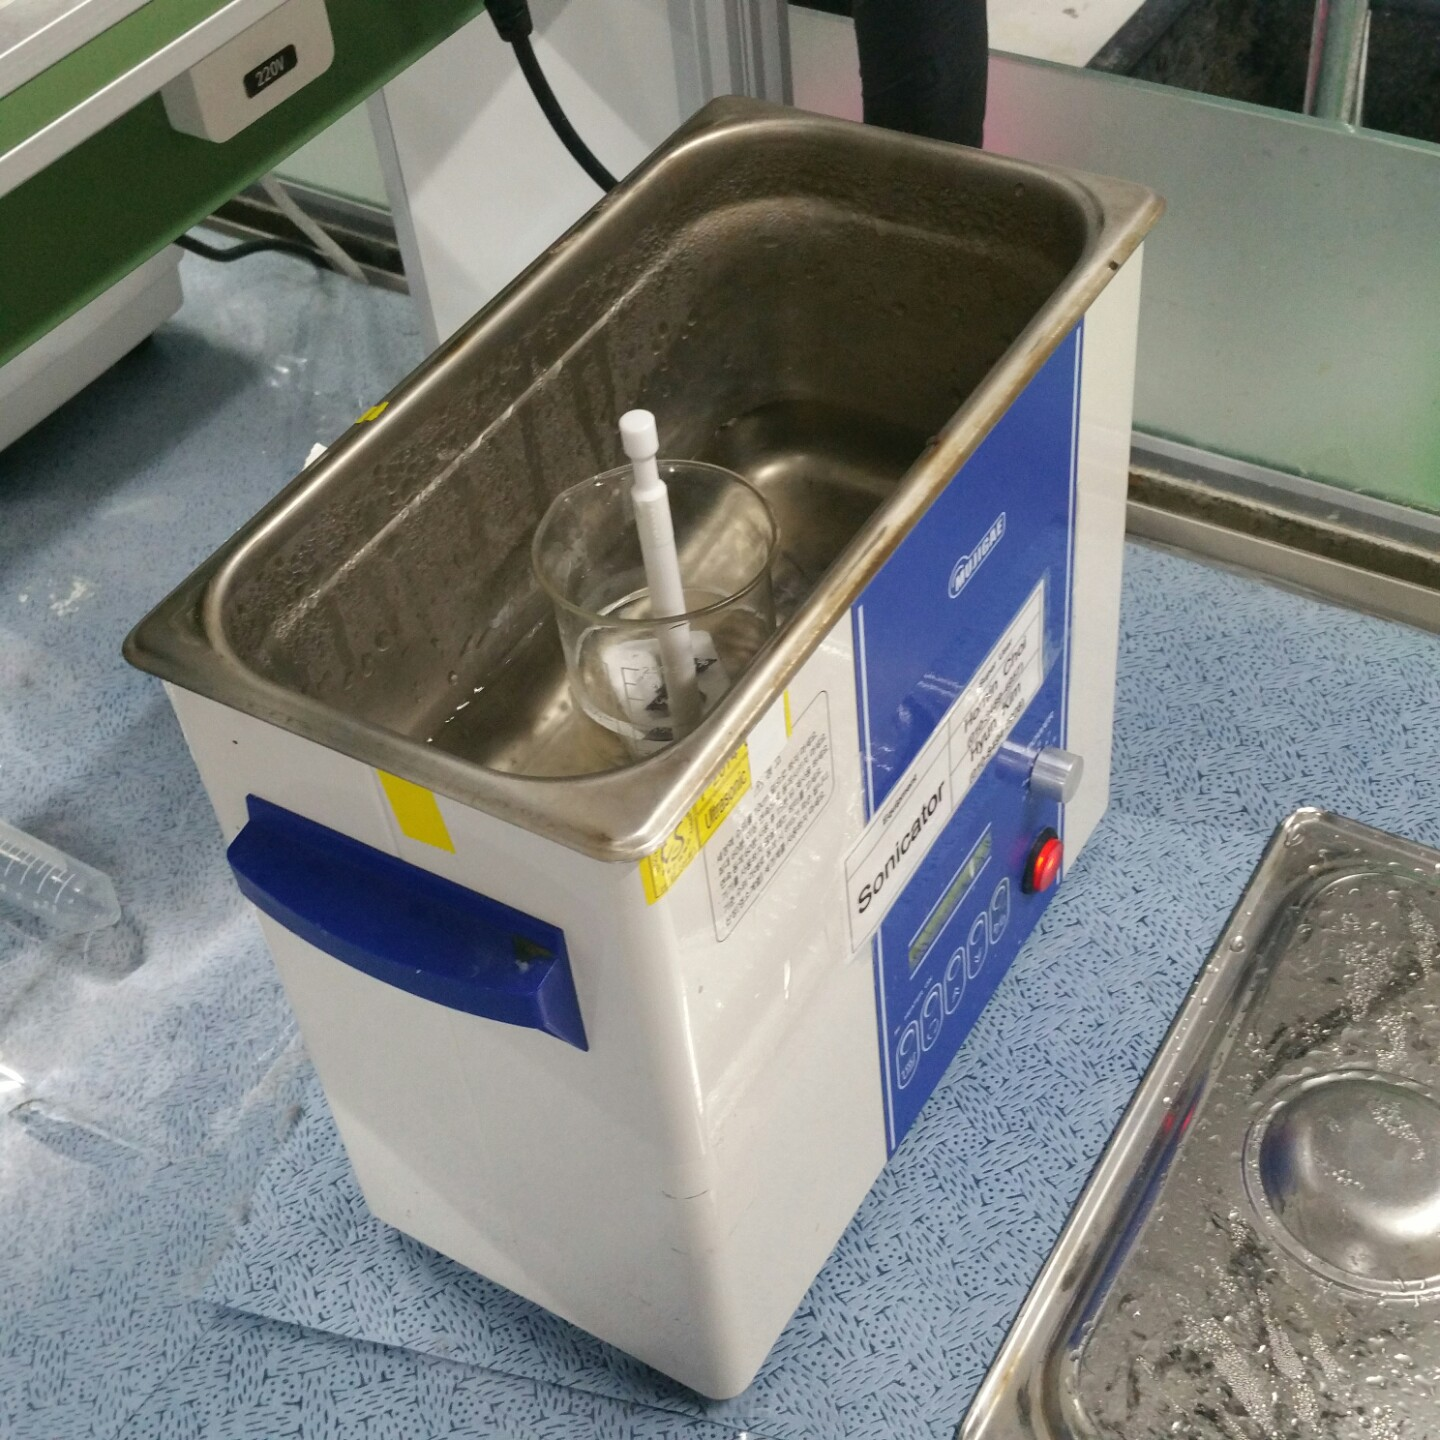
\includegraphics[width=0.3\textwidth]{sonicator}&
			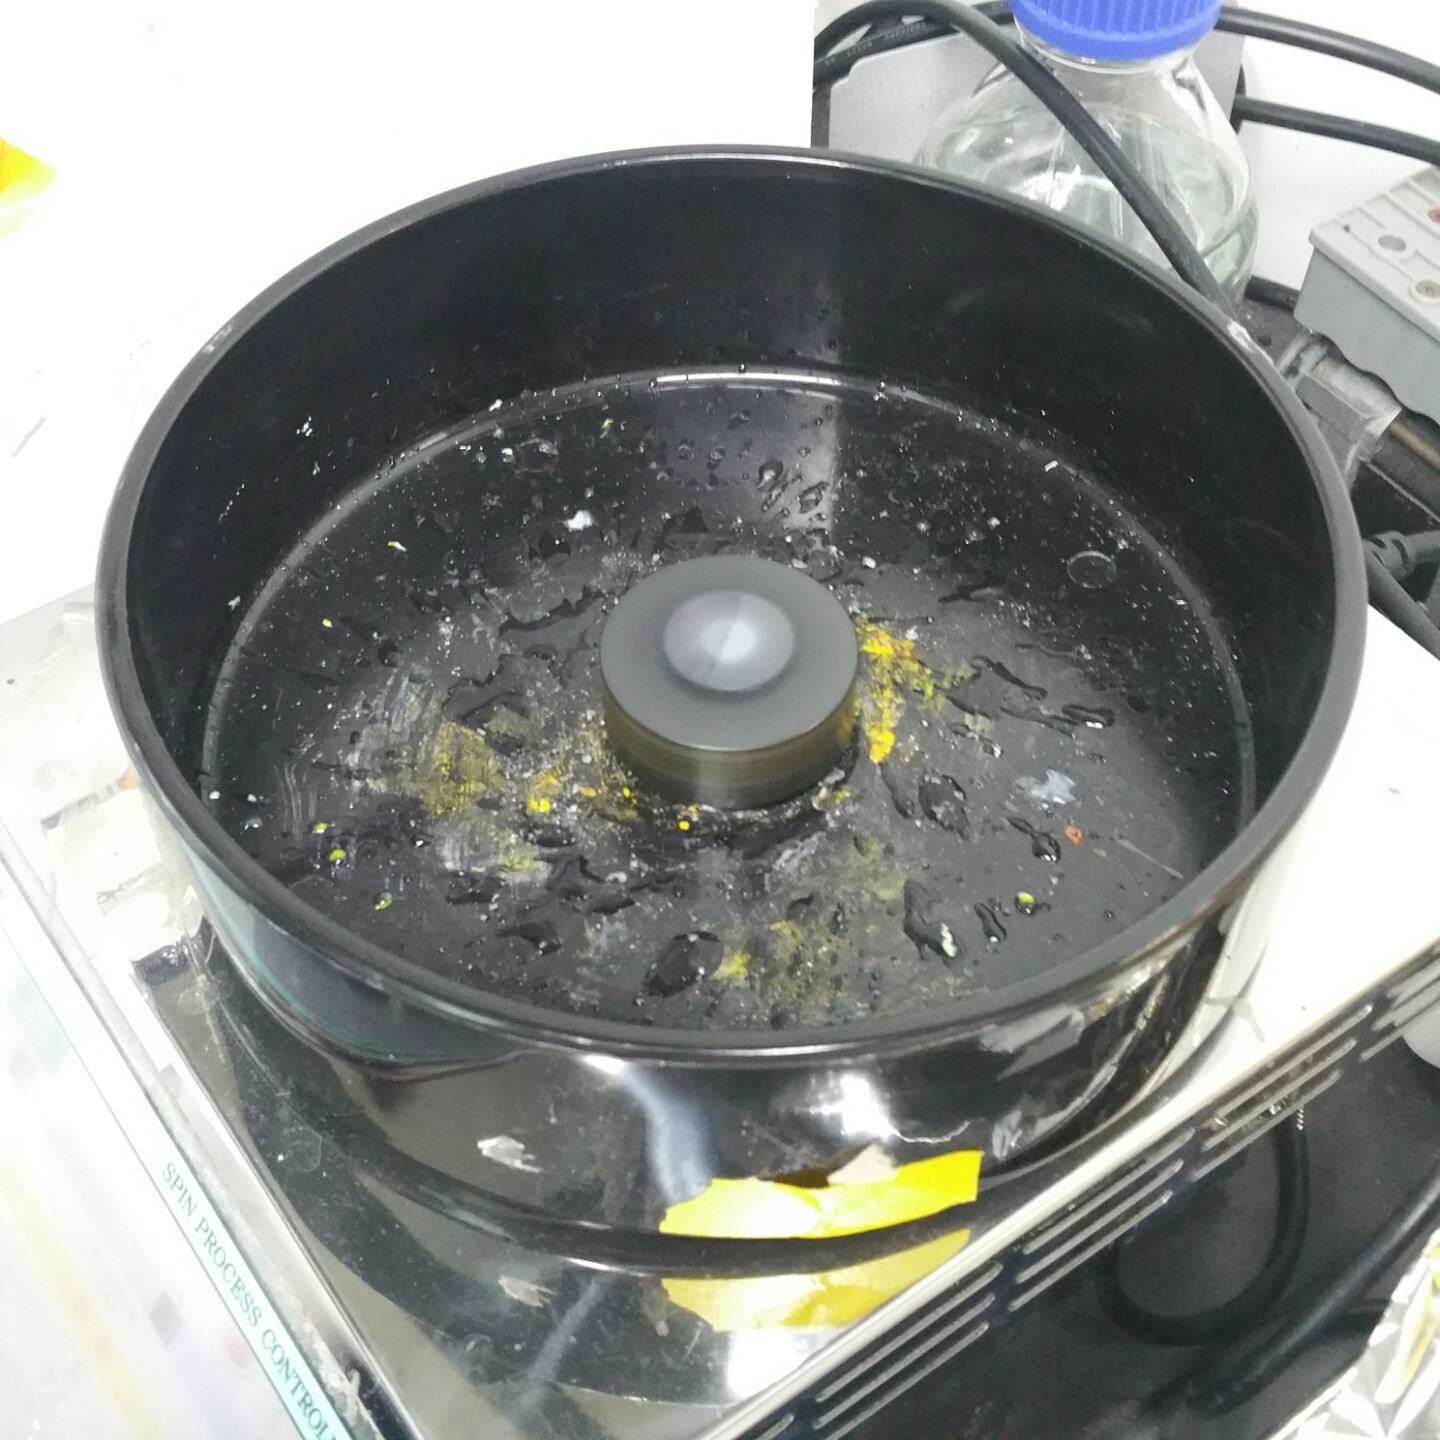
\includegraphics[width=0.3\textwidth]{spin_coating}&
			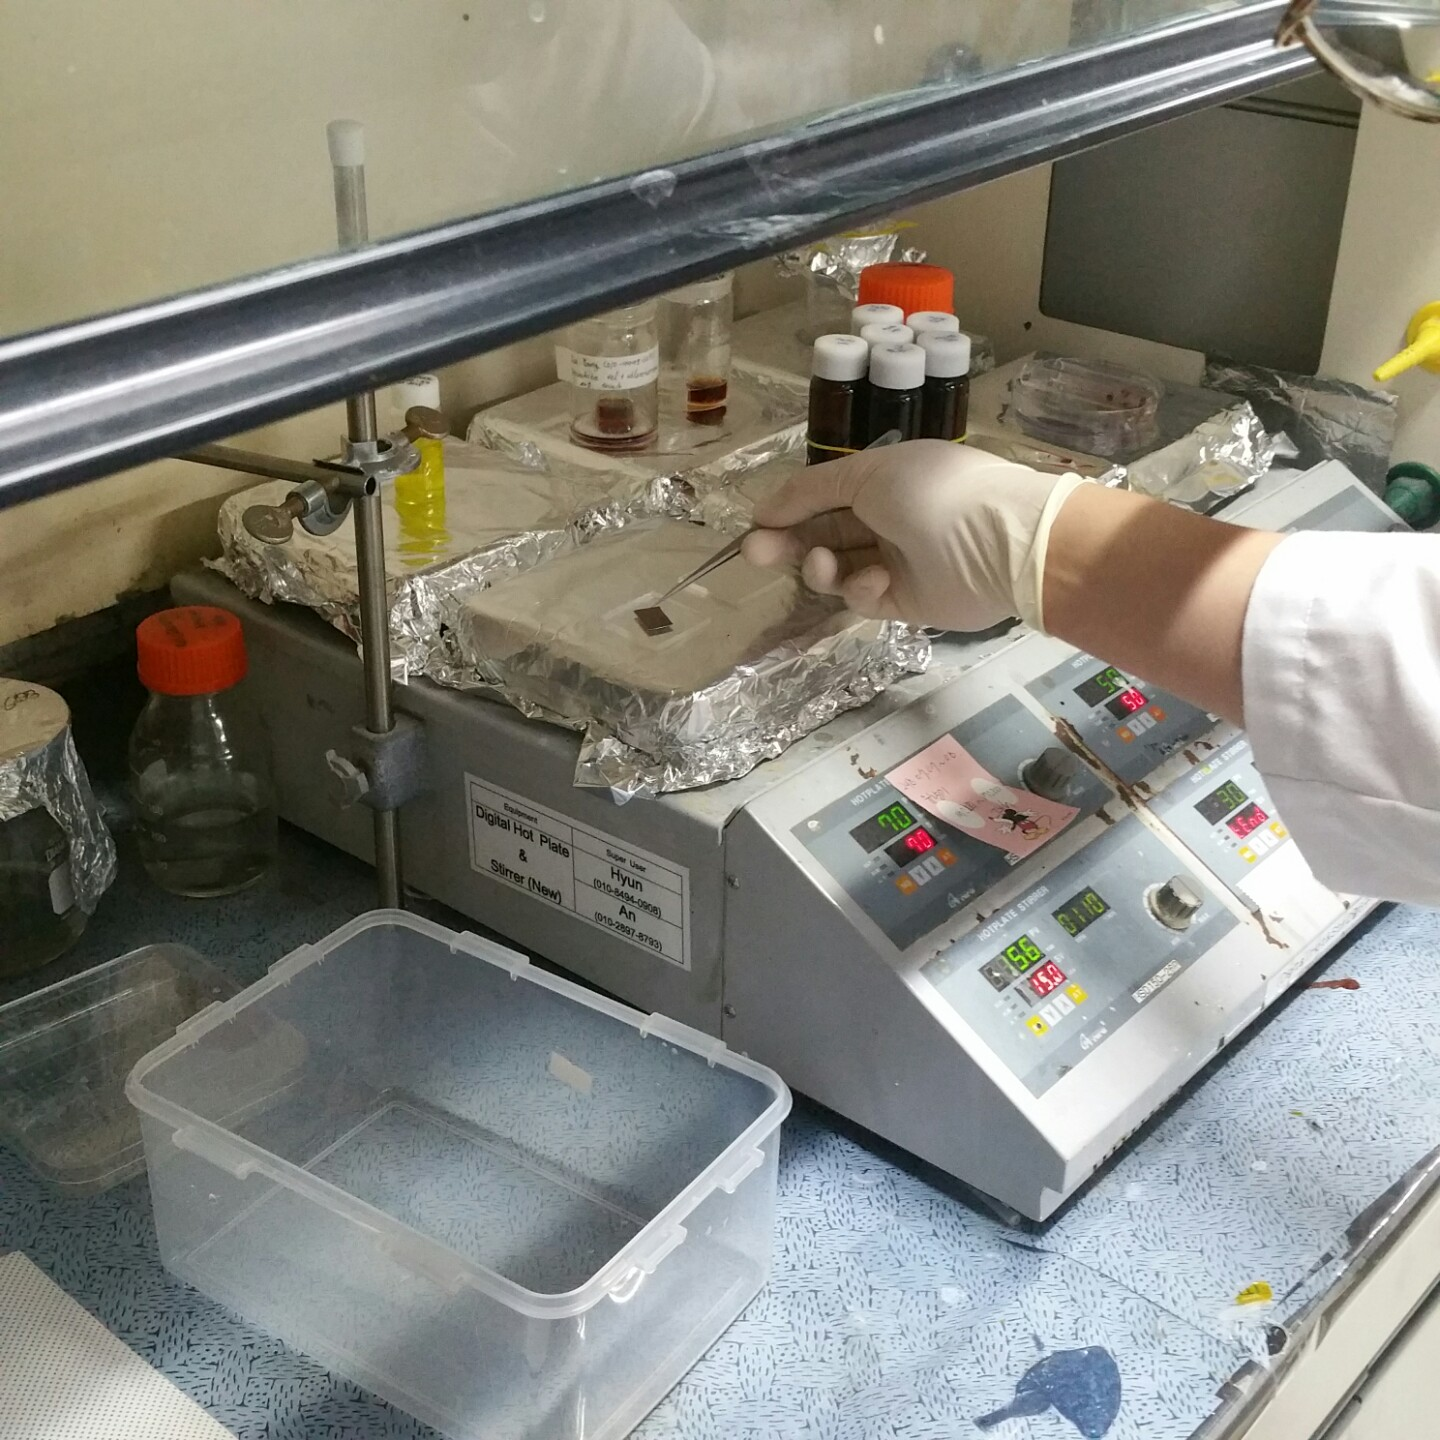
\includegraphics[width=0.3\textwidth]{hotplate}
		\end{tabular}
	\end{center}
	\begin{tikzpicture} [remember picture,overlay]
	\node[text=white] at (0.6, 4.7) {(a)};
	\node at (5.2, 4.7) {(b)};
	\node[text=white] at (10.1, 4.7) {(c)};
	\end{tikzpicture}	
	\caption{(a), (b), (c) correspond to following : sonicating, spin coating, PDMS stamping on hot plate.}
	\label{fig:sample}  
\end{figure}

Silicon wafer 위에 spin coating을 이용하여 용액을 균일하게 펼쳐주었다. 2000rpm으로 1분간 회전시켜주었고 미리 100도로 달궈놓았던 핫플레이트에서 5분간 PDMS를 이용하여 눌러주었다.

\begin{figure}[H]
	\begin{center}
		\begin{tabular}{cc}
			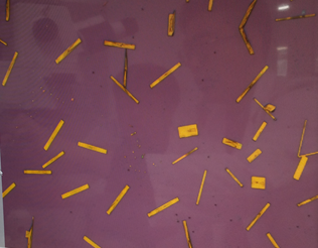
\includegraphics[width=0.45\textwidth]{OM}
		\end{tabular}
	\end{center}
	\caption{A silicon wafer taken with an OM (optical microscope).}
	\label{fig:om}  
\end{figure}
PDMS stamping 과정을 거친 이후에 silicon wafer에 결정이 잘 형성되었는지 확인하기 위해 OM(광학현미경)으로 1차적인 확인을 해주었다. 그 결과 Figure \ref{fig:om} 에서 잘 형성된 결정 여럿을 관찰할 수 있었고, 그 중 가장 잘 형성된 하나의 결정을 통해 연구를 진행하였다.

\subsection{데이터 추출}
제작된 sample을 NT-MDT 기기를 통하여 PL mapping 하였다. 생성된 단결정에 측정할 위치를 정해 놓고 PL을 측정하였다.  PL mapping이란, sample의 각 위치에서의 PL 데이터를 모두 담은 파일을 만드는 과정이다. 이 데이터는 레이저의 조리개를 $OD = 2$ 로 맞춰놓은 ND2 상태에서 측정하였다. 이렇게 만들어진 파일에서는 임의의 점에서의 PL data 를 얻어낼 수 있다는 장점이 있다.
\begin{figure}[H]
	\begin{center}
		\begin{tabular}{cc}
			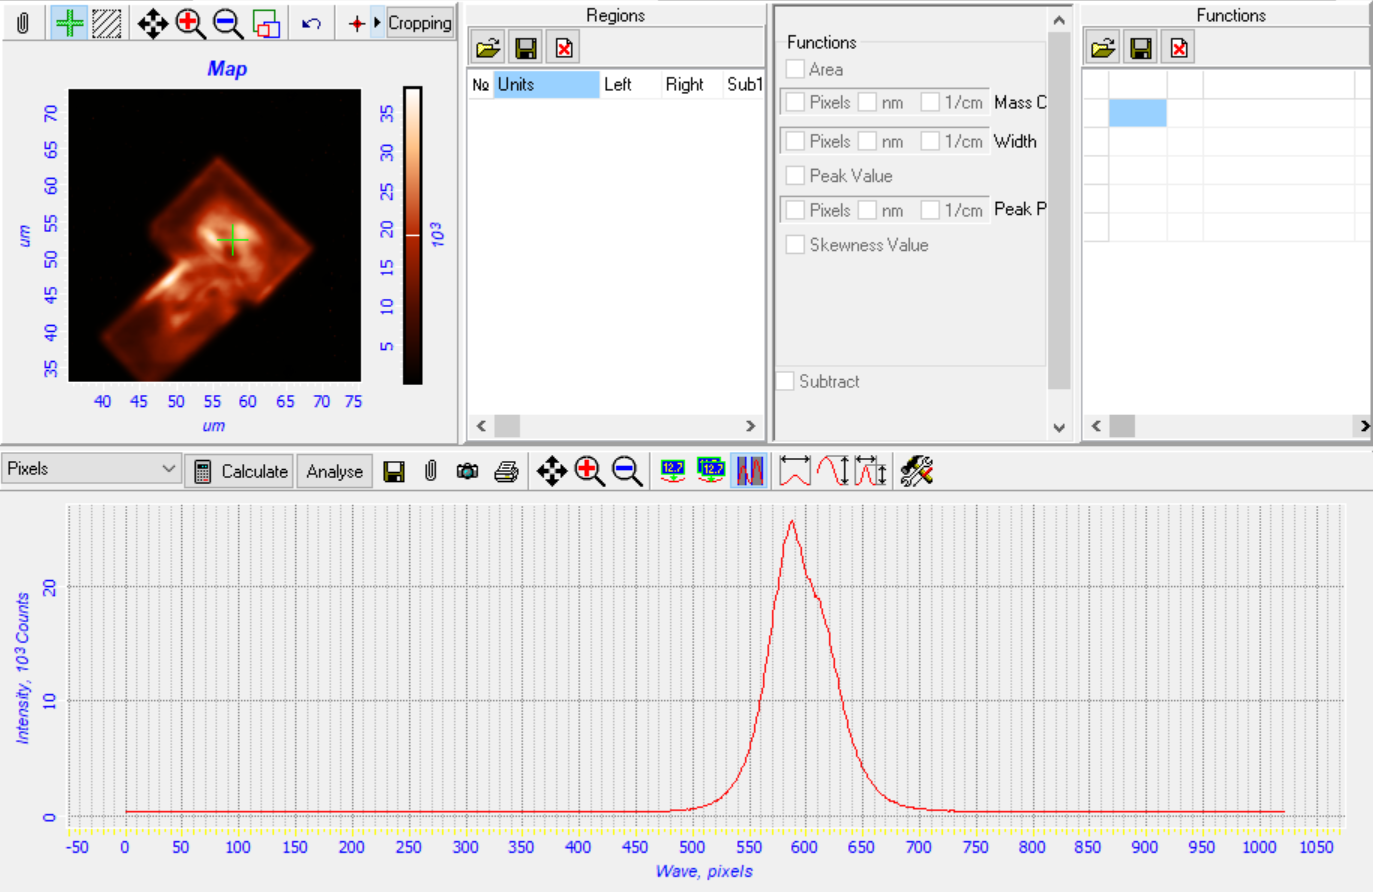
\includegraphics[width=0.65\textwidth]{Nova_screen_capture}&
			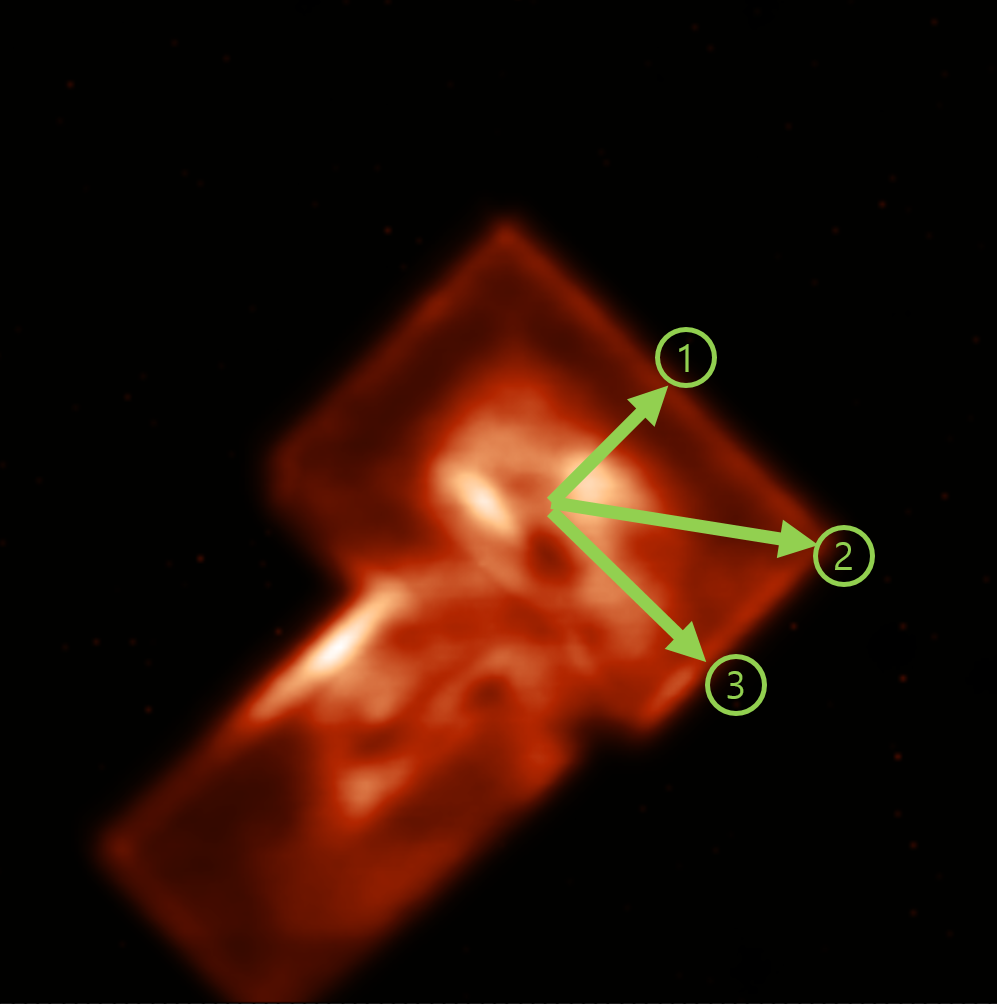
\includegraphics[width=0.4\textwidth]{line123}
		\end{tabular}
	\end{center}
	\begin{tikzpicture} [remember picture,overlay]
	\node at (0.6, 6.2) {(a)};
	\node[text=white] at (10.5, 6) {(b)};
	\end{tikzpicture}
	\caption{(a) shows extracting data by using Nova-Px program. We set the center point using the Nova-Px program and set the path as (b) based on that point.}
	\label{fig:nova}  
\end{figure}
Nova Px 프로그램을 활용하여 PL mapping 된 파일에서 데이터를 각 점 별로 뽑아내었다. Figure \ref{fig:nova}와 같은 화면에서 초록색 십자의 위치를 조절하여 원하는 위치의 PL peak을 얻어낼 수 있다. 중앙에서부터 바깥으로 나갈 때의 PL peak 의 경향성을 알아보기 위해 Figure \ref{fig:nova} 의 오른쪽 사진에서 볼 수 있는 1, 2, 3 경로의 데이터를 추출하였다.

중앙에서부터 바깥 쪽으로 나가는 경로에서의 PL data를 추출해낸다. 중앙으로 잡은 점의 좌표는 (59.0, 53.6, 33)이다. 이때 좌표를 (x, y, z) 라 했을 때 x, y는 사진상에서의 좌표, z는 그림에서 보이는 밝기의 크기, 즉 PL peak의 대략적인 상대적 크기이다. 그림 상으로는 정중앙이 아닐 수 있지만 PL peak이 가장 높게 나온 곳이므로 올바른 경향성을 찾아내기 위하여 설정 하였다. 설정된 중앙으로부터 바깥 방향으로 나가는 line 1, 2, 3 를 Table 1 과 같이 설정하였다.

\begin{table}[H]%[width=1.0\linewidth]
	\caption{Routing lines 1, 2, and 3}
	\label{table01}
	\centering
	\begin{tabular}{c c}
	\toprule
	경로 번호 & 경로\\
	\toprule
	Line 1 & (59.0, 53.6, 33)-->(62.3, 56.9, 14) / +(0.4, 0.4) 씩 8번, 점 9개\\
	Line 2 & (59.0, 53.6, 33)-->(68.0, 51.3, 13) / +(0.8, -0.2) 씩 11번, 점 12개\\
	Line 3 & (59.0, 53.6, 33)-->(64.7, 47.9, 17) / +(0.4, -0.4) 씩 14번, 점 15개\\
	\toprule
	\end{tabular}
	\end{table}
다
중앙으로 잡은 점을 point 0, 각 line에 대해 있는 점들을 point 1-1, 1-2, … , 1-8, 2-1, 2-1, … , 2-11, 3-1, 3-2, … , 3-14로 정의하였다. line 1 은 point 0 부터 point 1-8, line 2 은 point 0 부터 point 2-11, line 3 은 point 0 부터 point 3-14 까지 이다. 
\\

\subsection{분석 과정}
\subsubsection{point data peak fitting}
각 점들의 추출된 data를 분석하기 위해서 Origin 9 프로그램을 사용하였다. Chen (2018) 에 의하면 CsPbBr3 에서 biexciton과 exciton의 peak이 나타나는 wave length 는 각각 약 580nm, 600nm 이다\cite{chen2018room}. 이 사실을 바탕으로 PL data에서 보여진 peak을 두개의 peak의 합으로 fitting 하였다. Peak fitting 을 할 때에 Hartley (1961)의 gauss fitting 매커니즘을 프로그램에서 사용하였으며, biexciton 과 exciton이 존재하는 wave length에 peak 위치를 설정한 후 fitting을 진행하였다\cite{hartley1961modified}. Figure \ref{fig:point0}은 그 중 하나의 예시이다.

\begin{figure}[H]
	\begin{center}
		\begin{tabular}{cc}
			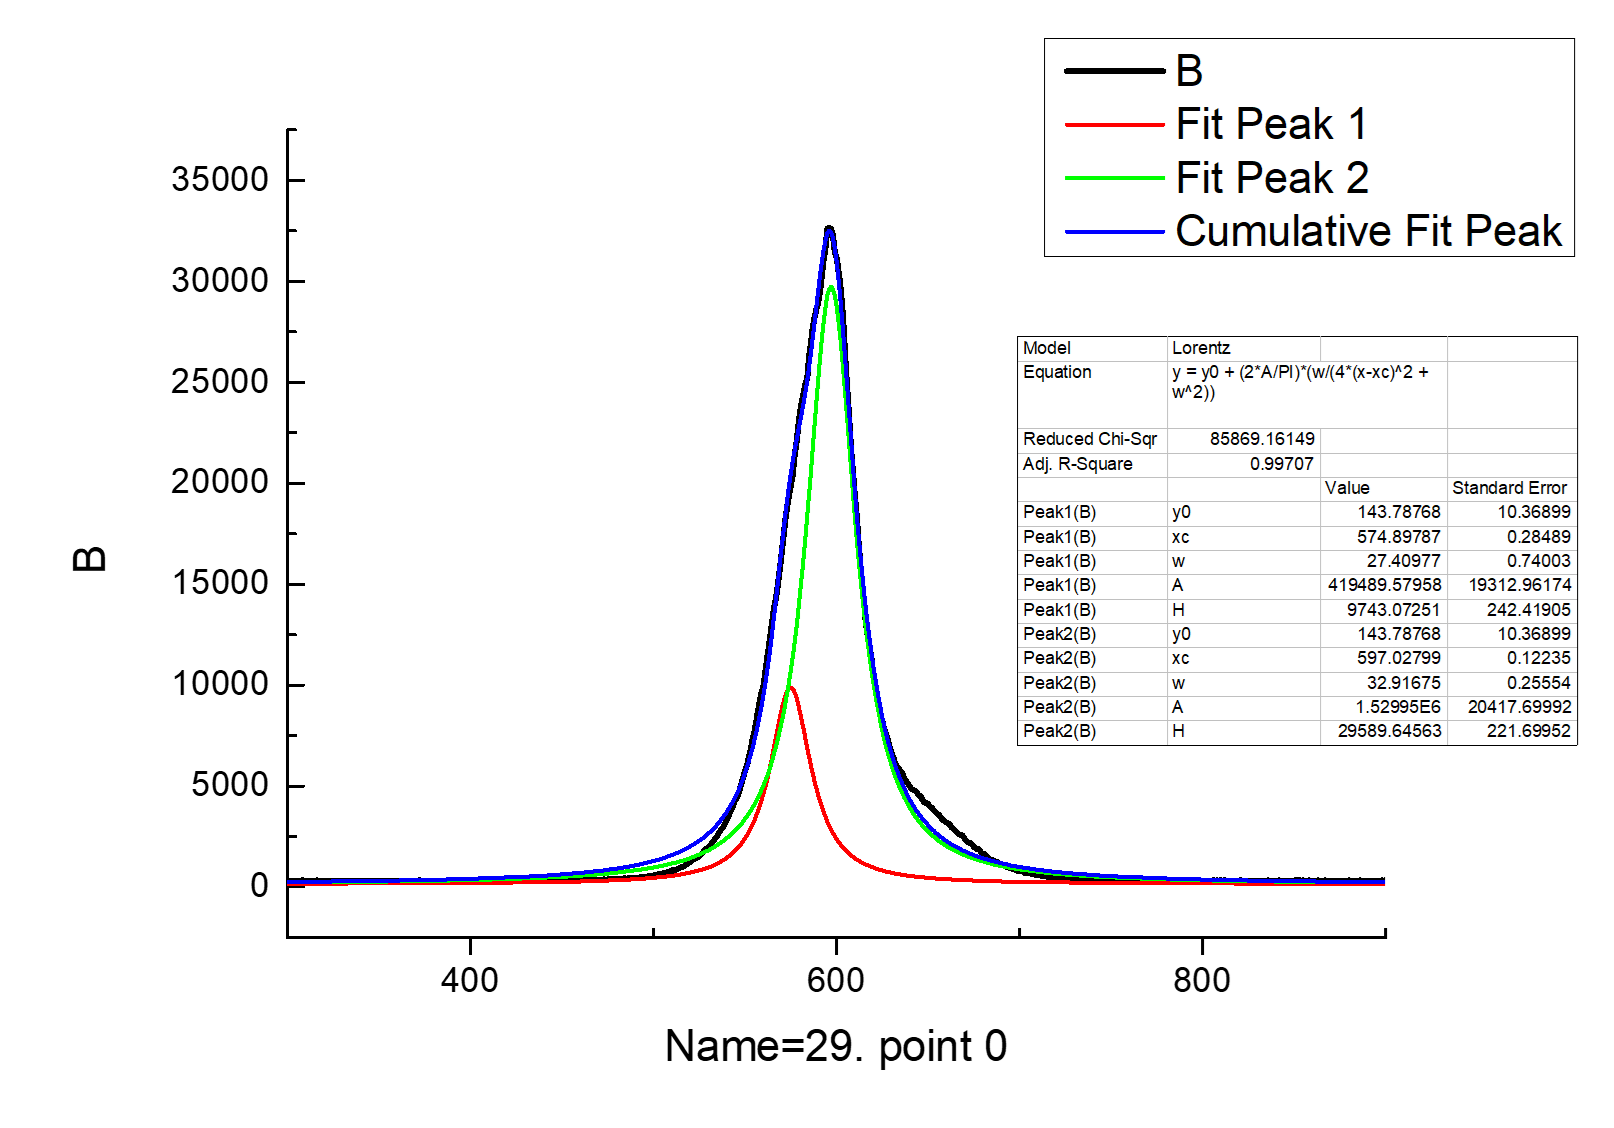
\includegraphics[width=0.8\textwidth]{point0}
		\end{tabular}
	\end{center}
	\caption{The PL data of the set point 0 is shown by sum of exciton and biexciton peak.}
	\label{fig:point0}  
\end{figure}

Figure \ref{fig:point0}\과 같이 multiple peak fitting 을 마친 후에는 각 peak의 x값, 즉 wavelength 값과 y값, 즉 intensity 값을 데이터로 기록한 후 분석하였다.

\subsubsection{line data analyze}
위의 과정에서 각 point 들의 data 에 대한 peak fitting 을 한 이후에 그 경향성을 보기 위해 필요한 과정이다. 분석하고자 하는 것은 중앙에서 바깥으로 가면서 peak intensity의 경향성이다. 이를 위해서 peak fitting 과정에서 얻은 데이터인 각 point 에서의 biexciton, exciton peak 의 intensity 값을 y축, point 번호를 x 축으로 설정하여  line 1, line 2, line 3 별로 막대그래프를 그려서 경향성을 볼 수 있었다.
\\

\subsection{분석 결과 및 해석}
Line 1, Line 2, Line 3 에서의 결과를 각각 Figure \ref{fig:line1}, Figure \ref{fig:line2}, Figure \ref{fig:line3}에 나타내었다.

\begin{figure}[H]
	\begin{tabular}{cc}
		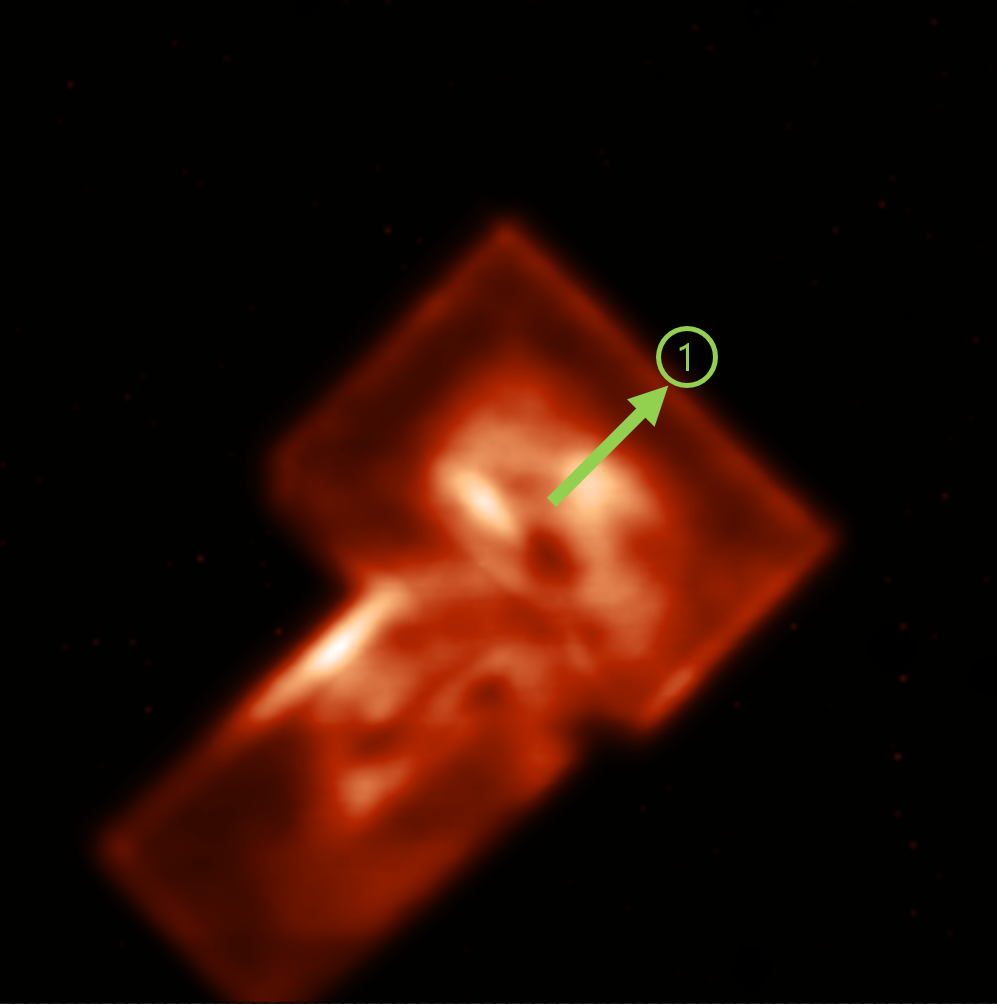
\includegraphics[width=0.3\textwidth]{line1}
		\begin{tikzpicture} [remember picture,overlay]	
		\node[text=white] at (-4, 4) {(a)};
		\end{tikzpicture}
		&
		\begin{tikzpicture}
		\begin{axis} [
		width=0.70\textwidth,%
		height = 5cm,%
		ybar,%
		bar width=5pt,
		title={Line 1},%
		xtick = data,%
		symbolic x coords={0, 1, 2, 3, 4, 5, 6, 7, 8},%
		ylabel= {Intensity(a.u.)},%
		ymin=0,ystep=5000,ymax=35000.0,%
		scaled y ticks = false,%
		ymajorgrids = true,
		legend style={at={(0.02,10)}},legend pos=north east]%
		\addplot table [x=no, y=biexciton] {./data/line1.csv}; %
		\addlegendentry {biexciton}%
		\addplot table [x=no, y=exciton] {./data/line1.csv}; %
		\addlegendentry {exciton}%
		\end{axis}
		\node at (-0.9, 3.5) {(b)};
		\end{tikzpicture}
	\end{tabular}
	\caption{(a) shows the route set to line 1. (b)  is the analyzed data and shows the tendency in the path along line 1.}
	\label{fig:line1}  
\end{figure}




Figure \ref{fig:line1}, 즉 line 1에서는 exciton과 biexciton 모두 감소하는 추세를 보이다가 끝에서 증가하는 모습을 볼 수 있다.

\begin{figure}[H]
	\begin{tabular}{cc}
		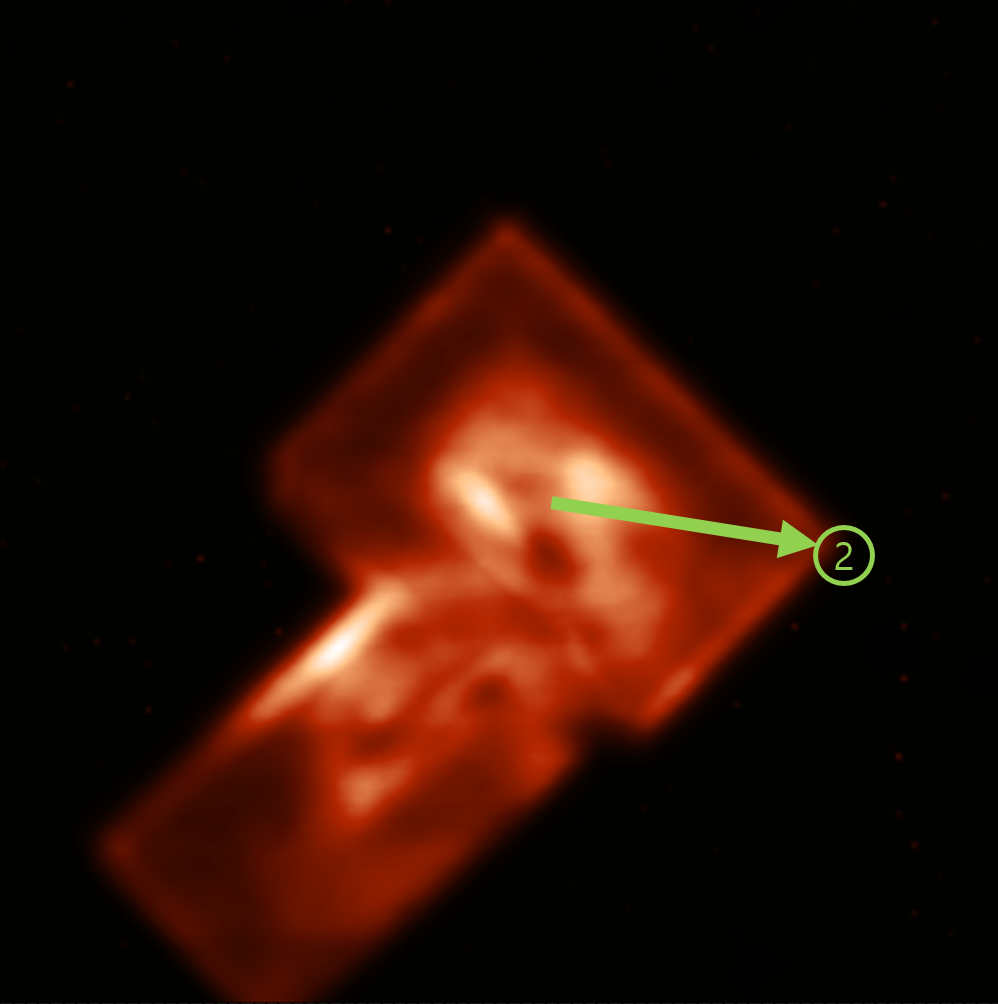
\includegraphics[width=0.3\textwidth]{line2}
		\begin{tikzpicture} [remember picture,overlay]	
		\node[text=white] at (-4, 4) {(a)};
		\end{tikzpicture}
		&
		\begin{tikzpicture}
		\begin{axis} [
		width=0.70\textwidth,%
		height = 5cm,%
		ybar,%
		bar width=5pt,
		title={Line 2},%
		xtick = data,%
		symbolic x coords={0, 1, 2, 3, 4, 5, 6, 7, 8, 9, 10, 11},%
		ylabel= {Intensity(a.u.)},%
		ymin=0,ystep=5000,ymax=35000.0,%
		scaled y ticks = false,%
		ymajorgrids = true,
		legend style={at={(0.02,10)}},legend pos=north east]%
		\addplot table [x=no, y=biexciton] {./data/line2.csv}; %
		\addlegendentry {biexciton}%
		\addplot table [x=no, y=exciton] {./data/line2.csv}; %
		\addlegendentry {exciton}%
		\end{axis}
		\node at (-0.9, 3.5) {(b)};
		\end{tikzpicture}
	\end{tabular}
	\caption{(a) shows the route set to line 2. (b)  is the analyzed data and shows the tendency in the path along line 2.}
	\label{fig:line2}  
\end{figure}


Figure \ref{fig:line2}, 즉 line 2에서는 exciton과 biexciton 모두 감소하는 추세를 보이다가 가장 끝 두점에서는 biexciton은 급격히 증가, exciton은 급격히 감소함을 볼 수 있다.

\begin{figure}[H]
	\begin{tabular}{cc}
		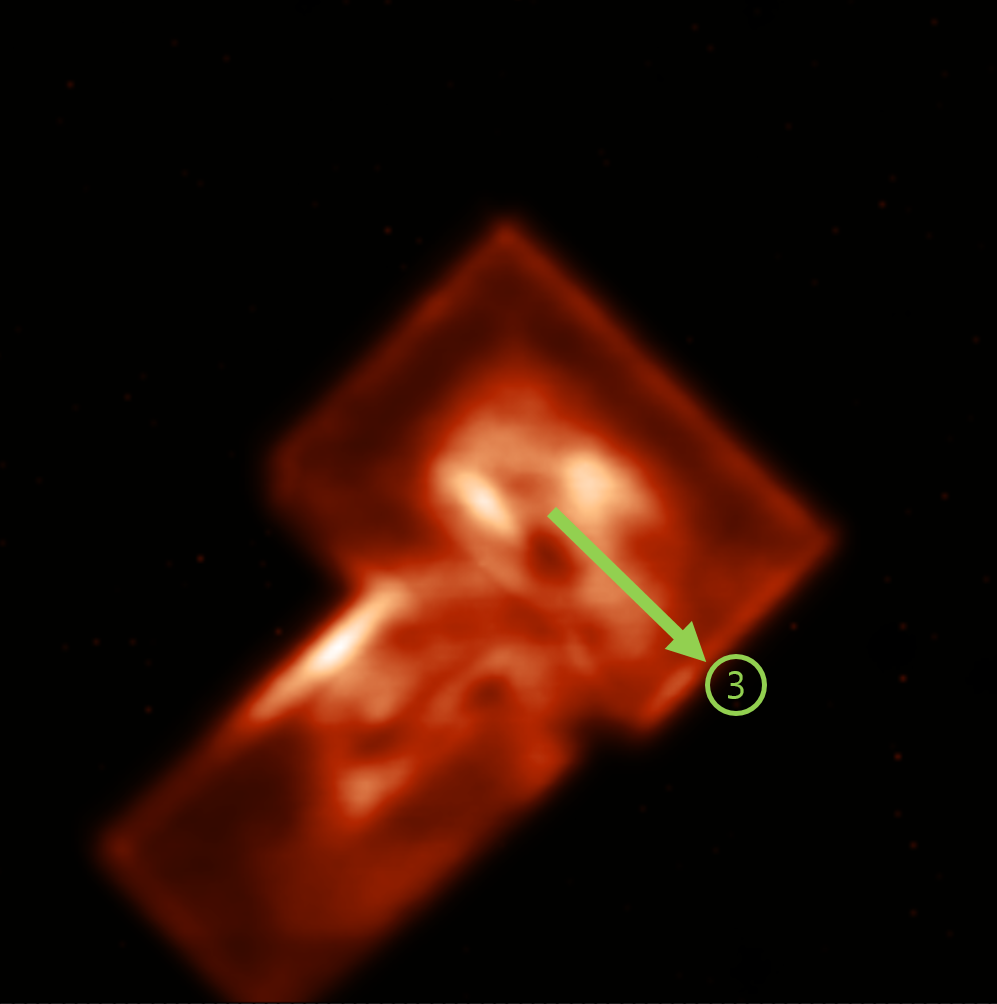
\includegraphics[width=0.3\textwidth]{line3}
		\begin{tikzpicture} [remember picture,overlay]	
		\node[text=white] at (-4, 4) {(a)};
		\end{tikzpicture}
		&
		\begin{tikzpicture}
		\begin{axis} [
		width=0.70\textwidth,%
		height = 5cm,%
		ybar,%
		bar width=5pt,
		title={Line 3},%
		xtick = data,%
		symbolic x coords={0, 1, 2, 3, 4, 5, 6, 7, 8, 9, 10, 11, 12, 13, 14},%
		ylabel= {Intensity(a.u.)},%
		ymin=0,ystep=5000,ymax=35000.0,%
		scaled y ticks = false,%
		ymajorgrids = true,
		legend style={at={(0.02,10)}},legend pos=north east]%
		\addplot table [x=no, y=biexciton] {./data/line3.csv}; %
		\addlegendentry {biexciton}%
		\addplot table [x=no, y=exciton] {./data/line3.csv}; %
		\addlegendentry {exciton}%
		\end{axis}
		\node at (-0.9, 3.5) {(b)};
		\end{tikzpicture}
	\end{tabular}
	\caption{(a) shows the route set to line 3. (b)  is the analyzed data and shows the tendency in the path along line 3.}
	\label{fig:line3}  
\end{figure}





Figure \ref{fig:line3} , 즉 line 3에서는 exciton은 감소, biexciton은 증가하는 추세를 보이다가 가장 끝 두점에서는 biexciton은 급격히 감소, exciton은 급격히 증가함을 볼 수 있다.

세 line에서 exciton, biexciton 각각의 공통되는 경향성이나 규칙은 찾아보기 어렵다. 하지만 중앙에서 중간까지 갈 때는 특정한 경향성을 보이는 듯 하다가 가장 바깥, 가장자리에서 그 경향성이 반대가 되는 모습을 볼 수 있다. 종합적으로 보았을 때에는 가장자리로 가면서 감소하는 모습을 보이다가 다시 증가하는 모습이 세 line모두에서 나타났다.


	